\documentclass[12pt,a4paper]{article}

% ── Packages ──────────────────────────────────────────────
\usepackage[utf8]{inputenc}
\usepackage[T1]{fontenc}
\usepackage{lmodern}
\usepackage[margin=2.5cm]{geometry}
\usepackage{graphicx}
\usepackage{xcolor}
\usepackage{listings}
\usepackage{hyperref}
\usepackage{booktabs}
\usepackage{float}
\usepackage{enumitem}
\usepackage{caption}
\usepackage{parskip}
\usepackage{fancyhdr}
\usepackage{titlesec}

% ── Colors ────────────────────────────────────────────────
\definecolor{codeblue}{RGB}{26,54,93}
\definecolor{codegray}{RGB}{100,100,100}
\definecolor{codegreen}{RGB}{22,101,52}
\definecolor{codepurple}{RGB}{128,0,128}
\definecolor{backcolor}{RGB}{248,250,252}
\definecolor{stringcolor}{RGB}{163,21,21}

% ── Code Listing Style ───────────────────────────────────
\lstdefinestyle{codestyle}{
    backgroundcolor=\color{backcolor},
    commentstyle=\color{codegreen},
    keywordstyle=\color{codeblue}\bfseries,
    stringstyle=\color{stringcolor},
    basicstyle=\ttfamily\scriptsize,
    breakatwhitespace=false,
    breaklines=true,
    captionpos=b,
    keepspaces=true,
    showspaces=false,
    showstringspaces=false,
    showtabs=false,
    tabsize=2,
    frame=single,
    rulecolor=\color{codegray!30},
    xleftmargin=1em,
    framexleftmargin=0.5em,
    numbers=left,
    numberstyle=\tiny\color{codegray},
    numbersep=8pt,
}
\lstset{style=codestyle}

% TypeScript language definition for listings
\lstdefinelanguage{TypeScript}{
  keywords={const, let, var, function, return, if, else, for, while, do, switch, case, break, continue, new, try, catch, throw, typeof, instanceof, in, of, class, extends, implements, interface, type, enum, import, export, from, default, as, async, await, yield, true, false, null, undefined, void, never, any, string, number, boolean, object},
  sensitive=true,
  comment=[l]{//},
  morecomment=[s]{/*}{*/},
  morestring=[b]",
  morestring=[b]',
  morestring=[b]`,
}

% ── Section Styling ───────────────────────────────────────
\titleformat{\section}{\Large\bfseries\color{codeblue}}{\thesection}{1em}{}
\titleformat{\subsection}{\large\bfseries\color{codeblue!80}}{\thesubsection}{1em}{}
\titleformat{\subsubsection}{\normalsize\bfseries\color{codeblue!60}}{\thesubsubsection}{1em}{}

% ── Header / Footer ──────────────────────────────────────
\pagestyle{fancy}
\fancyhf{}
\fancyhead[L]{\small\textit{Sakny — University Housing Platform}}
\fancyhead[R]{\small\textit{Frontend Implementation}}
\fancyfoot[C]{\thepage}
\renewcommand{\headrulewidth}{0.4pt}

% ── Document ─────────────────────────────────────────────
\begin{document}

% ══════════════════════════════════════════════════════════
% TITLE
% ══════════════════════════════════════════════════════════
\begin{center}
    {\LARGE\bfseries\color{codeblue} Frontend Implementation}\\[0.5em]
    {\large Sakny — University Housing Platform}\\[1em]
    \rule{0.6\textwidth}{0.5pt}
\end{center}

\tableofcontents
\newpage

% ══════════════════════════════════════════════════════════
% SECTION 1: INTRODUCTION & TECHNOLOGY STACK
% ══════════════════════════════════════════════════════════
\section{Introduction \& Technology Stack}

The Sakny frontend constitutes the primary user-facing engine of the university housing platform. Architecturally, it is designed to manage two asymmetric portal workflows while maintaining a unified, performant, and secure client-side runtime:
\begin{itemize}
    \item \textbf{Student Portal:} Focuses on intuitive user experiences (UX) designed to guide students through housing discovery, apartment filtering, bilingual applications, real-time message exchange with managers, document submission, and payment tracking.
    \item \textbf{Admin Portal:} Focuses on data density and high operational speed. It provides administrators with visual dashboards to oversee application workflows, automate room allocations, manage maintenance tickets, and track campus analytics.
\end{itemize}

Rather than developing these portals as separate codebases, they are unified in a single monolithic frontend codebase. This unification ensures maximum reuse of design systems, translation dictionaries, and core services while enforcing complete segregation of view logic and security boundaries.

\subsection{Technology Stack Selection \& Technical Justifications}

To support these complex requirements, the technologies selected represent a modern, robust, and highly optimized frontend architecture. Table 1 outlines the specific components, followed by an in-depth justification of their technical roles.

\begin{table}[H]
\centering
\begin{tabular}{@{}llp{7.5cm}@{}}
\toprule
\textbf{Technology} & \textbf{Version} & \textbf{Technical Role \& Architectural Justification} \\
\midrule
Next.js & 16.2.4 & High-performance React framework. Selected for its App Router (file-system-based nesting), React Server Components (RSC) execution model, build-time static generation, and automated SEO optimization APIs. \\
React & 19.2.4 & Component lifecycle engine, managing state synchronization, lightweight virtual DOM reconciliation, and standard client-side interactivity. \\
TypeScript & 5.x & Strict static type checking layer. Prevents compile-time anomalies, enforces API contract schemas, and establishes reliable refactoring boundaries. \\
Tailwind CSS & 4.x & Utility-first styling compiler. Offers a local custom theme configuration that generates lightweight, atomic styles at compile-time with zero client-side evaluation cost. \\
Material Symbols & — & Scalable, customizable vector icon library loaded via Google Fonts CDN, minimizing overall assets footprint. \\
PostCSS & — & CSS preprocessing engine used by Tailwind CSS v4 to resolve dependencies and optimize bundles. \\
\bottomrule
\end{tabular}
\caption{Frontend technology stack.}
\end{table}

\subsubsection{Architectural Decoupling: Next.js App Router vs. Traditional Alternatives}

The decision to utilize Next.js (App Router) instead of a standard Single Page Application (SPA) compiler (e.g., Vite + React Router) or the legacy Next.js Pages Router was driven by three technical paradigms:
\begin{enumerate}[leftmargin=2em]
    \item \textbf{React Server Components (RSC):} In a traditional client-side SPA, the browser must download the entire JavaScript bundle, parse it, execute it, and then perform client-side fetching to show content. This causes a slow First Contentful Paint (FCP) and significant Time to Interactive (TTI). RSCs reverse this process. By default, Next.js App Router components execute on the server. The server compiles the static layout structure to clean HTML/CSS and streams it to the browser. Only interactive leaves containing the \texttt{"use client"} directive ship JavaScript to the client. This dramatically decreases the JavaScript bundle size, reducing memory consumption on mobile devices.
    \item \textbf{Dynamic Layout Preservation:} The App Router introduces physical directories containing nested layouts. When navigating between adjacent child pages (e.g., from student profile to catalog), only the page container is unmounted. The parent layout (hosting the sidebar, user context, and notification polling loop) remains completely mounted, avoiding redundant re-renders, preventing layout flashing, and preserving persistent client-side state.
    \item \textbf{Built-in Compilation Abstractions:} Next.js provides out-of-the-box build configurations for code-splitting (automatically splitting JS chunks per route), image optimization, font optimization, and SEO metadata generation, which would otherwise require hundreds of lines of complex Webpack or Vite configurations.
\end{enumerate}

\subsubsection{Compile-Time Security: TypeScript 5.x}

In a platform managing sensitive administrative workflows and student data, runtime failures due to undefined values or invalid API responses are unacceptable. TypeScript compiles code statically, converting potential runtime errors into compiler issues. It enforces strict type parameters across all components, hooks, and services. By typing the API responses (using generic TypeScript boundaries), components are statically aware of the exact keys returned by the backend, reducing standard runtime anomalies.

\subsubsection{Styling Efficiency: Tailwind CSS 4.x and PostCSS}

Traditional CSS methodologies like CSS Modules or CSS-in-JS (e.g., \texttt{styled-components}) introduce performance bottlenecks. CSS-in-JS requires active JavaScript execution at runtime to parse styles and inject them into the DOM, which degrades frame rates during page transitions. Tailwind CSS v4 solves this by parsing utility classes at compile-time. The compiler analyzes the JSX templates and generates a highly optimized, atomic CSS bundle. If a class is not used, it is excluded, resulting in a production stylesheet under 15 KB.

PostCSS acts as the compilation pipeline, translating modern custom theme rules, nested rules, and imports into standard, cross-browser compliant CSS.

% ══════════════════════════════════════════════════════════
% SECTION 2: PROJECT STRUCTURE
% ══════════════════════════════════════════════════════════
\section{Project Structure \& File Organization}

The directory organization follows a strict \textbf{separation of concerns} pattern designed to keep the codebase maintainable as the project scales. By isolating system layers, the team can refactor business logic without affecting page layouts or styling systems.

\begin{lstlisting}[language={},title={Project folder structure}]
src/
|-- app/                    # Routing & Composition Layer (Next.js App Router)
|   |-- layout.tsx          # App Root (Fonts, contexts, global HTML)
|   |-- page.tsx            # Main Landing page
|   |-- auth/               # Access Portal (Login, registration routing)
|   |-- dashboard/          # Student Portal routing (14 sub-routes)
|   |-- admin/              # Admin Portal routing (13 sub-modules)
|-- components/             # Stateless UI & State-Composition Components
|   |-- ui/                 # Atomic design system primitives (stateless)
|   |-- auth/               # Compound elements specific to login/register
|   |-- dashboard/          # Layout modules (Sidebars, context-bars, steppers)
|   |-- admin/              # Admin sidebar layout and table components
|-- services/               # Centralized Data Fetching Layer (API clients)
|   |-- api.ts              # Custom Fetch abstraction with auth and error boundaries
|-- hooks/                  # Abstracted Browser & React Hook API logic
|   |-- useScrollReveal.ts  # IntersectionObserver trigger for animation states
|-- i18n/                   # Global Context Internationalization
    |-- LanguageContext.tsx  # Dynamic translation context provider
    |-- useTranslation.ts   # Context access hook
    |-- locales/            # Localization dictionary mapping (EN, AR)
\end{lstlisting}

\subsection{Separation of Concerns and Modular Data Flows}

The structural design decouples data fetching, UI representation, and localization, preventing overlapping responsibilities:
\begin{itemize}[leftmargin=2em]
    \item \textbf{Page Decoupling:} Pages inside the \texttt{app/} folder do not house complex UI layouts or business logic. They serve as composition roots. They mount layout frames, inject static metadata, and load high-level feature components. This separation allows developers to refactor a component's visual style without risking routing failures.
    \item \textbf{Domain-Isolated Components:} Reusable components are split into two categories. Primitives (in \texttt{ui/}) are strictly stateless and design-driven (e.g., inputs, buttons, cards). Feature components (e.g., \texttt{auth/}, \texttt{dashboard/}) wrap these primitives with specific local state and actions. Domain grouping prevents naming collisions and keeps the component folder structure logical.
    \item \textbf{Single-Point API Abstraction:} The entire codebase communicates with the REST backend via the isolated `api.ts` file in \texttt{services/}. No React component is allowed to invoke the native global browser \texttt{fetch()} function directly. Centralizing HTTP calls guarantees that authentication header injections, base URL overrides, and network exceptions are handled in a single, predictable location.
\end{itemize}

\subsection{Runtime Data Flow Mechanics}

The workflow below illustrates the step-by-step lifecycle when a user interacts with the interface:

\begin{enumerate}
    \item \textbf{Routing:} The browser hits a URL (e.g., \texttt{/dashboard/catalog}). Next.js loads the matching route layout in \texttt{app/dashboard/layout.tsx} followed by the page in \texttt{app/dashboard/catalog/page.tsx}.
    \item \textbf{Component Mounting:} The catalog page mounts the search and house list components. The translation system (\texttt{i18n/LanguageContext}) translates the placeholder text based on the active locale.
    \item \textbf{Data Request:} Inside a React hook lifecycle, a service client call is executed: \texttt{apiClient("/housing/catalog")}.
    \item \textbf{Token Injection:} The custom API wrapper catches the call, injects the user's JWT bearer token from \texttt{localStorage}, and fires the request over HTTP to the backend.
    \item \textbf{Response Resolution:} The promise resolves. The API wrapper inspects the response code. If correct, it returns a typed structure \texttt{\{ success: true, data: [...] \}} back to the component, which updates its local state and triggers a React render cycle to draw the listings.
\end{enumerate}

% ══════════════════════════════════════════════════════════
% SECTION 3: DESIGN SYSTEM & STYLING
% ══════════════════════════════════════════════════════════
\section{Design System \& Styling Approach}

To present a professional, modern visual aesthetic, the Sakny platform implements a cohesive design system rather than relying on ad-hoc styles. This system is driven by \textbf{semantic design tokens} and modern CSS architectures.

\subsection{Design Tokens and Semantic Styling}

Tailwind CSS v4 introduces a streamlined theme configuration system declared directly in \texttt{globals.css}. By assigning colors and typography to variables inside the `@theme` directive, the styling compiler creates a unified, semantic styling language.

\begin{lstlisting}[language=TypeScript,title={globals.css — Custom design tokens}]
@import "tailwindcss";

@theme {
  --color-primary: #1A365D;                  
  --color-primary-container: #152c4d;        
  --color-accent-yellow: #FBBF24;            
  --color-background: #F8FAFC;              
  --color-surface: #ffffff;                 

  --color-status-available: #166534;         
  --color-status-limited: #a16207;           
  --color-status-full: #991b1b;              

  --font-headline: "Manrope", sans-serif;
  --font-body: "Public Sans", sans-serif;

  --shadow-soft: 0 4px 20px -2px rgba(0, 0, 0, 0.05);
  --shadow-soft-lg: 0 10px 30px -5px rgba(0, 0, 0, 0.08);
}
\end{lstlisting}

\subsubsection{Technical Role of Semantic Tokens}

Declaring semantic colors directly in the CSS compiler theme plays an essential architectural role:
\begin{itemize}[leftmargin=2em]
    \item \textbf{Semantic Identity Definition:} The core role of these semantic tokens is to define the platform's visual identity. Instead of styling components with arbitrary, hardcoded design colors like \texttt{text-[\#1A365D]}, components are styled using functional terms like \texttt{text-primary} and \texttt{bg-surface}.
    \item \textbf{Structural Decoupling and Global Scalability:} This separation decouples styling rules from the raw HTML structure. If the university decides to change its official color palette, the modification is isolated to the single `@theme` block in \texttt{globals.css}. The build engine compiles the new hex values throughout the entire portal without requiring edits to individual components.
    \item \textbf{PostCSS Compilation and CSS Variable Resolution:} The PostCSS compiler parses the `@theme` block, converting the token keys into native CSS Custom Properties (e.g., \texttt{--color-primary}) bound to the root DOM node. When Tailwind class strings are loaded in the browser, the browser resolves the variable names dynamically. This enforces design consistency across different layout levels (e.g., using \texttt{bg-background} for parent layouts, and elevated \texttt{bg-surface} for nested cards).
\end{itemize}

\subsection{Typography Optimization \& Performance}

Typography utilizes two modern font families to balance visual appeal and readability:
\begin{itemize}
    \item \textbf{Manrope:} Chosen for high-impact headlines and UI navigation markers due to its geometric styling and balance.
    \item \textbf{Public Sans:} A highly readable, clean sans-serif typeface designed for body copies, tabular datasets, and user forms.
\end{itemize}

These fonts are loaded using the \texttt{next/font} system inside \texttt{layout.tsx}:

\begin{lstlisting}[language=TypeScript,title={layout.tsx — Optimized font loading}]
const manrope = Manrope({
  subsets: ["latin"],
  variable: "--font-headline",
  display: "swap",
});

const publicSans = Public_Sans({
  subsets: ["latin"],
  variable: "--font-body",
  display: "swap",
});
\end{lstlisting}

\subsubsection{Addressing Performance \& Layout Shifts}

Using the built-in \texttt{next/font} compiler utility addresses critical web performance metrics:
\begin{itemize}[leftmargin=2em]
    \item \textbf{Performance-Oriented Asset Delivery:} The role of this typography configuration is to deliver smooth font rendering across different operating systems while minimizing network requests during initial page loads.
    \item \textbf{Prevention of Layout Shifts and Flash of Unstyled Text:} Standard font loading configurations cause Flash of Invisible Text (FOIT) or Flash of Unstyled Text (FOUT) while the browser downloads custom assets over the network. This causes the page layout to shift when the font renders, resulting in a poor user experience and reducing the Cumulative Layout Shift (CLS) score.
    \item \textbf{Compile-Time Bundling and Swap Optimization Lifecycle:} Next.js downloads Google Font assets at build time and embeds them locally within the application bundle. The browser does not need to send external HTTP requests to Google Fonts CDNs at runtime. By injecting the \texttt{display: "swap"} parameter, the compiler configures the CSS \texttt{@font-face} declarations with \texttt{font-display: swap}. This instructs the browser to immediately render a system fallback font (e.g., Arial) while the local web font downloads in the background, smoothly swapping in the optimized font once ready. Next.js automatically calculates size-adjust parameters for the fallbacks, preventing annoying content shifts when the swap occurs.
\end{itemize}

\subsection{Custom GPU-Accelerated Visual Utilities}

To implement professional UI elements like floating layouts and overlay headers, the design features custom CSS utility modifiers:

\begin{lstlisting}[language=TypeScript,title={Custom utility configurations}]
@utility glass-nav {
  background-color: rgba(255, 255, 255, 0.9);
  backdrop-filter: blur(16px);
  -webkit-backdrop-filter: blur(16px);
}
\end{lstlisting}

\subsubsection{Technical Performance of GPU Filters}
\begin{itemize}[leftmargin=2em]
    \item \textbf{Translucent Interface Layering:} The role of this utility is to provide a modern, translucent frosted-glass styling for floating headers, maintaining text readability when scrolling over rich background images.
    \item \textbf{Mitigation of Main Thread Execution Bottlenecks:} Traditional blur effects rely on heavy JavaScript recalculations or canvas drawing techniques that run on the main CPU thread, which can degrade frame rates. The custom utility uses modern CSS properties to offload rendering to the hardware graphics card.
    \item \textbf{Hardware-Accelerated Compositing Layer Processing:} The PostCSS compiler translates the `@utility glass-nav` declaration into standard CSS. When applied, the browser isolates the layout boundaries of the navbar, allocating a dedicated GPU composition layer. The hardware graphics card then applies a box blur filter to the pixels directly behind the container in real time, maintaining high scroll performance.
\end{itemize}

% ══════════════════════════════════════════════════════════
% SECTION 4: ROUTING & PAGE MANAGEMENT
% ══════════════════════════════════════════════════════════
\section{Routing \& Page Management}

The core architecture of Next.js relies on a \textbf{file-system-based routing} paradigm known as the App Router. The directory structure inside the `src/app/` folder dictates the routing map.

\subsection{Physical Routing Layout Map}

Figure 1 details the routing flow and access branches of the application:

\begin{figure}[H]
    \centering
    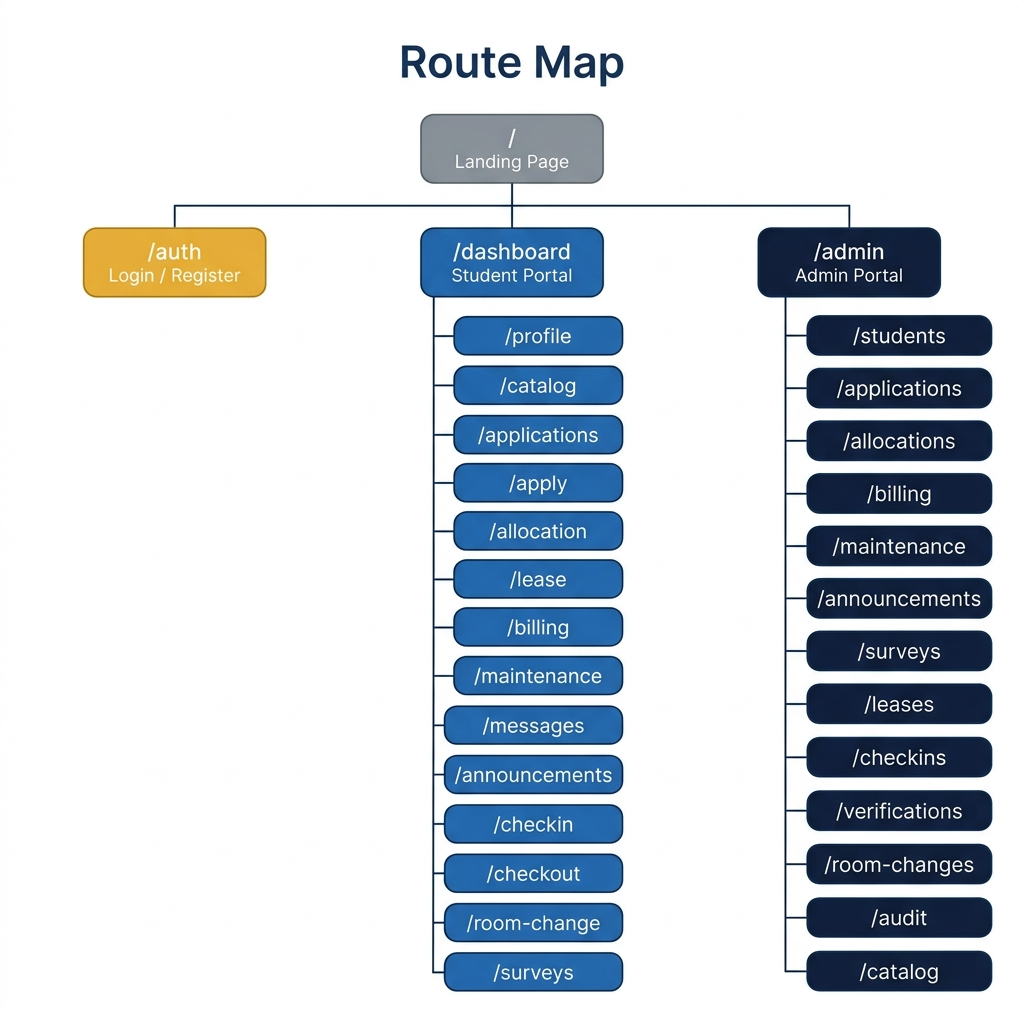
\includegraphics[width=\textwidth]{images/route_map_diagram.png}
    \caption{Complete route map of the Sakny frontend application.}
\end{figure}

The platform handles 30+ dynamic routes, categorized into three distinct operational domains:

\begin{table}[H]
\centering
\small
\begin{tabular}{@{}lll@{}}
\toprule
\textbf{Route Pattern} & \textbf{Operational Space} & \textbf{Technical Purpose} \\
\midrule
\texttt{/} & Public Domain & Landing page, platform marketing, and general information. \\
\texttt{/auth} & Public Gate & Unified login and sign-up interfaces. \\
\texttt{/dashboard} & Student Portal & Home view displaying application states and alert banners. \\
\texttt{/dashboard/profile} & Student Portal & Form-driven interface to manage personal information and upload documents. \\
\texttt{/dashboard/catalog} & Student Portal & Real-time housing browser with map integrations. \\
\texttt{/dashboard/applications} & Student Portal & Interactive table tracking the workflow phases of active applications. \\
\texttt{/dashboard/messages} & Student Portal & Interface for direct messaging with administrators. \\
\texttt{/dashboard/billing} & Student Portal & Payment receipts, fees tracking, and checkout operations. \\
\texttt{/admin} & Admin Portal & Home dashboard hosting analytic charts and system overviews. \\
\texttt{/admin/students} & Admin Portal & Table displaying student profiles, actions, and search metrics. \\
\texttt{/admin/applications} & Admin Portal & Dashboard for reviewing and approving student housing submissions. \\
\texttt{/admin/maintenance} & Admin Portal & System to process, categorize, and update maintenance tickets. \\
\bottomrule
\end{tabular}
\caption{Key routes distribution.}
\end{table}

\subsection{Nested Layout Architecture}

The App Router supports nested layouts. A parent layout (\texttt{layout.tsx}) wraps all sub-page directories, allowing shared UI structures to remain active across route changes.

\begin{figure}[H]
    \centering
    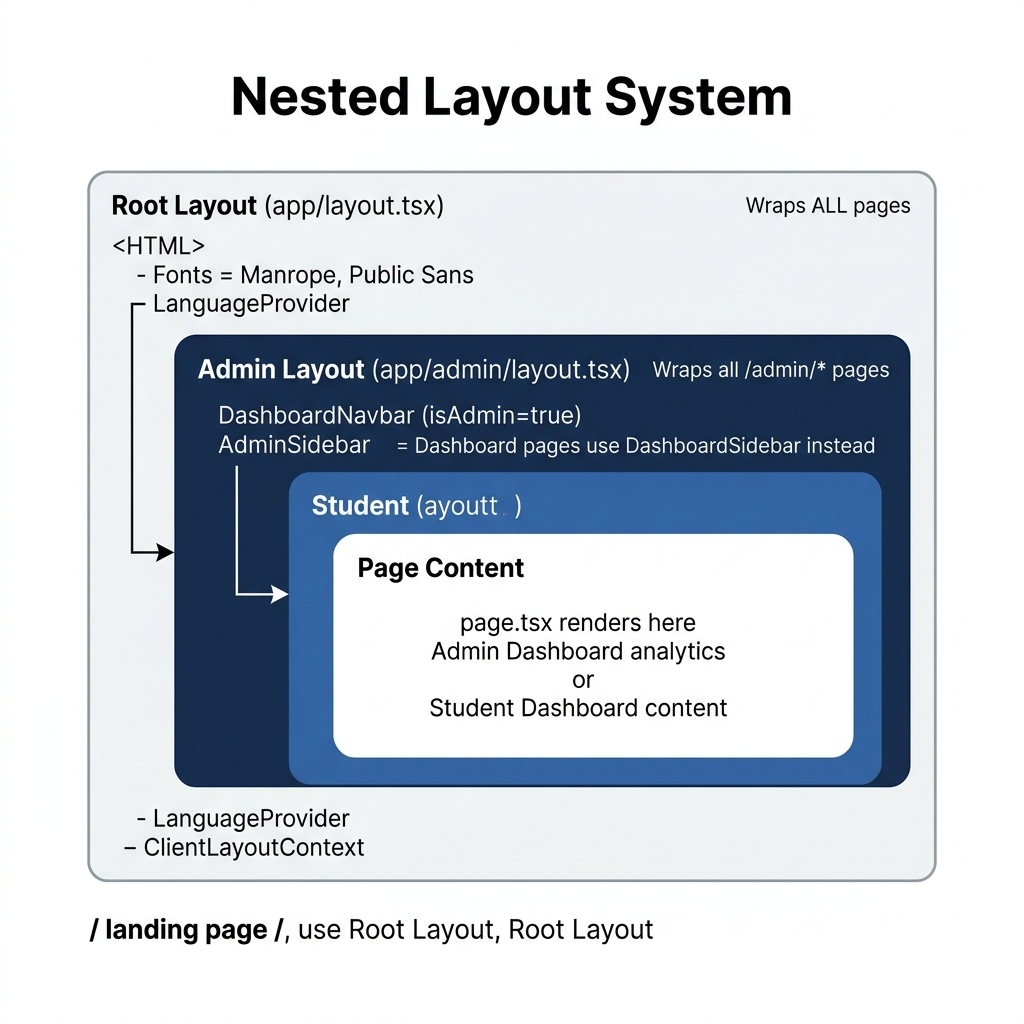
\includegraphics[width=0.85\textwidth]{images/nested_layouts.png}
    \caption{Nested layout inheritance — Root Layout wraps all pages, Admin Layout adds sidebar and navbar.}
\end{figure}

The \textbf{Root Layout} (\texttt{app/layout.tsx}) establishes global contexts, styles, and locale configurations:

\begin{lstlisting}[language=TypeScript,title={Root layout — Context wrapping pattern}]
export default function RootLayout({ children }: { children: React.ReactNode }) {
  return (
    <html lang="en" className={`${manrope.variable} ${publicSans.variable}`}>
      <body className="antialiased min-h-screen bg-background text-primary">
        <LanguageProvider>
          <ClientLayoutContext>
            {children}
          </ClientLayoutContext>
        </LanguageProvider>
      </body>
    </html>
  );
}
\end{lstlisting}

The \textbf{Admin Layout} (\texttt{app/admin/layout.tsx}) wraps all sub-routes under \texttt{/admin/*}. It mounts the admin sidebar and header structure while maintaining the inner view:

\begin{lstlisting}[language=TypeScript,title={Admin nested layout}]
export default function AdminLayout({ children }: { children: React.ReactNode }) {
  return (
    <div className="min-h-screen flex flex-col bg-background">
      <DashboardNavbar isAdmin />
      <div className="flex flex-1 relative">
        <AdminSidebar />
        <main className="lg:ml-64 pt-24 pb-12 px-8 flex-grow transition-all duration-300">
          {children}
        </main>
      </div>
    </div>
  );
}
\end{lstlisting}

\subsubsection{Technical Role and Mechanics of Nested Layouts}

Nested layouts provide three main technical advantages:
\begin{itemize}[leftmargin=2em]
    \item \textbf{UI Context Shell Preservation:} The role of layout structures is to isolate the persistent framework (such as sidebars, headers, and context providers) from the dynamic child pages, maintaining UI context during navigations.
    \item \textbf{State Preservation and Navigation Context Continuity:} In traditional single-page apps, route changes unmount the entire page tree, which destroys client-side states (e.g., active navigation highlights, sidebar scroll positions, and running background polling loops). Nested layouts preserve these persistent shells, preventing jarring layout shifts and layout flashing.
    \item \textbf{Selective Virtual DOM Subtree Re-rendering:} Next.js uses an optimized routing tree. When navigating between adjacent child pages (e.g., from student profile to catalog), only the page container is unmounted. The parent layout (hosting the sidebar, user context, and notification polling loop) remains completely mounted, avoiding redundant re-renders, preventing layout flashing, and preserving persistent client-side state.
\end{itemize}

\subsection{Server Components vs. Client Components Execution Model}

A core benefit of the App Router is its hybrid rendering model:
\begin{itemize}[leftmargin=2em]
    \item \textbf{React Server Components (RSC):} By default, every page and component inside `src/app/` is compiled as a Server Component. It has direct access to server-side resources, cannot hold state variables (\texttt{useState}), and does not run JavaScript in the client's browser. This minimizes the initial bundle size.
    \item \textbf{Client Components (CC):} If a component needs user interactivity, browser APIs (such as local storage or window event listeners), or lifecycle hooks (\texttt{useState}, \texttt{useEffect}), it is marked as a Client Component by placing the \texttt{"use client"} directive at the very top of the file.
\end{itemize}

This boundary model ensures that static structural parts (such as landing page grids, section footers, or routing layout containers) remain pure Server Components, while only interactive elements (such as login forms, navigation toggles, or map interfaces) ship JavaScript to the client.

% ══════════════════════════════════════════════════════════
% SECTION 5: REUSABLE COMPONENT DESIGN
% ══════════════════════════════════════════════════════════
\section{Reusable Component Design}

The component architecture is modeled as a \textbf{three-tier composition system} designed to maximize design consistency, maintainability, and testing efficiency.

\begin{figure}[H]
    \centering
    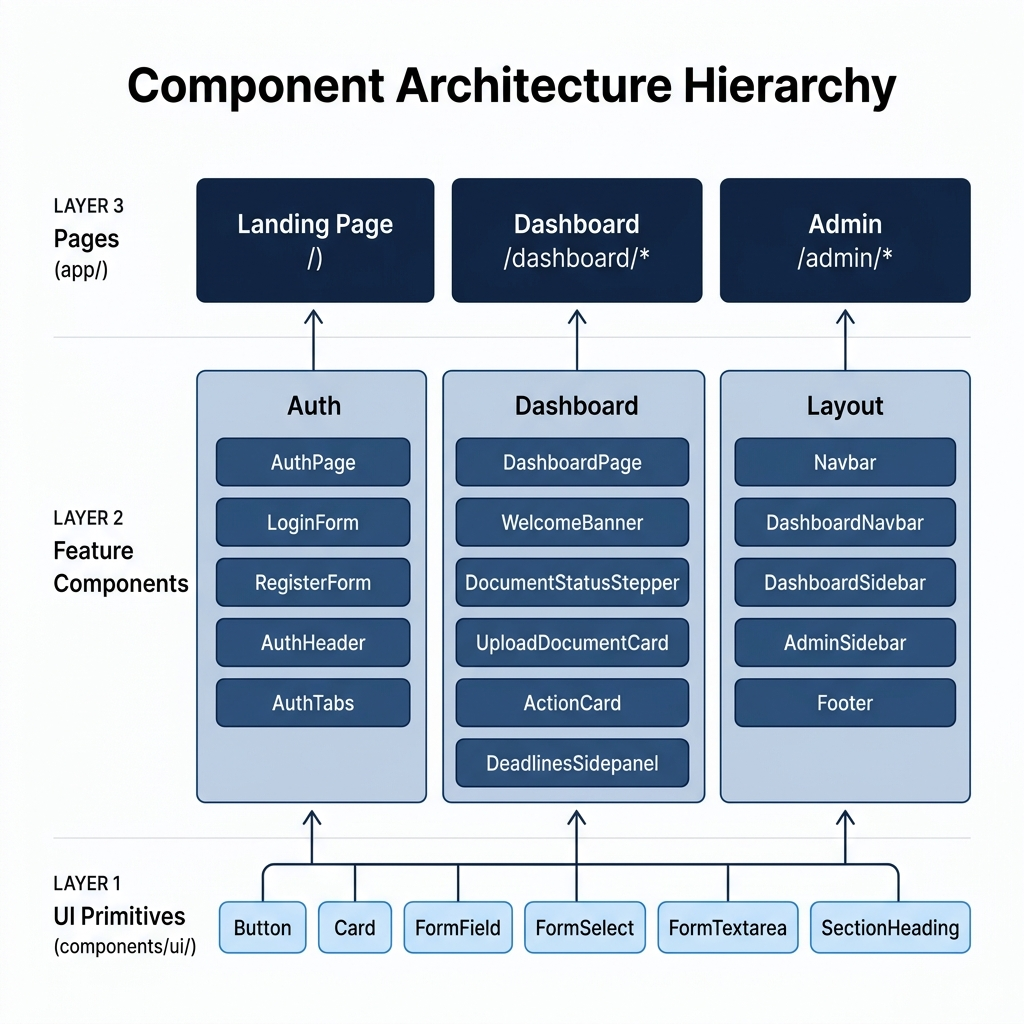
\includegraphics[width=\textwidth]{images/component_hierarchy.png}
    \caption{Component hierarchy — primitives compose into feature components, which compose into pages.}
\end{figure}

\subsection{Composition Architecture Layers}
\begin{enumerate}
    \item \textbf{UI Primitives (Tier 1):} Located in \texttt{components/ui/}. These atomic components (Buttons, Cards, Input FormFields) are stateless, design-token focused, and contain no domain knowledge. They focus entirely on visual presentation, accessible HTML markup, and style transitions.
    \item \textbf{Feature Components (Tier 2):} These compound components (e.g., \texttt{LoginForm}, \texttt{CatalogFilter}, \texttt{UploadCard}) combine multiple Tier 1 primitives, wire up local states or contexts, and execute API calls.
    \item \textbf{Page Composition (Tier 3):} Located in the `app/` folder. The parent page file loads multiple Tier 2 components and structures them within responsive grids.
\end{enumerate}

\subsection{UI Primitives Core Specification}

The system defines six core Tier 1 primitives, which are reused to build every view in the application:

\begin{table}[H]
\centering
\begin{tabular}{@{}llp{7cm}@{}}
\toprule
\textbf{Primitive Name} & \textbf{API Interface / Key Props} & \textbf{Visual and Practical Purpose} \\
\midrule
\texttt{Button} & \texttt{variant}, \texttt{icon}, \texttt{iconPosition} & Action trigger supporting color configurations (Primary, Secondary, Outline, Navy) and transition animations. \\
\texttt{Card} & \texttt{icon}, \texttt{title}, \texttt{description} & Visual container displaying information with support for interactive hover elevations. \\
\texttt{FormField} & \texttt{label}, \texttt{icon}, \texttt{error}, \texttt{type} & Standardized text input, integrating validation states, password toggling, and RTL alignments. \\
\texttt{FormSelect} & \texttt{label}, \texttt{options}, \texttt{error} & Dynamic dropdown select input for controlled lists. \\
\texttt{FormTextarea} & \texttt{label}, \texttt{error} & Multi-line text input for feedback or descriptions. \\
\texttt{SectionHeading} & \texttt{title}, \texttt{subtitle} & Unified typographic treatment for section headers. \\
\bottomrule
\end{tabular}
\caption{UI primitives system.}
\end{table}

\subsubsection{Technical Teardown: The \texttt{Button} Primitive \& Variant Mapping Pattern}

The `Button` component showcases an optimized visual styling pattern: mapping semantic styles to key-value maps to keep the component clean and performant.

\begin{lstlisting}[language=TypeScript,title={Button.tsx — Variant map pattern}]
import React from "react";

type ButtonProps = React.ButtonHTMLAttributes<HTMLButtonElement> & {
  variant?: "primary" | "secondary" | "outline" | "navy";
  icon?: string;
  iconPosition?: "left" | "right";
};

export const Button: React.FC<ButtonProps> = ({
  variant = "primary",
  icon,
  iconPosition = "right",
  children,
  className = "",
  ...props
}) => {
  const baseStyles = "transition-all duration-300 font-label flex items-center justify-center gap-2";
  
  const variants = {
    primary: "bg-accent-yellow text-primary px-10 py-5 rounded-xl font-bold text-lg hover:bg-accent-yellow-hover hover:scale-105 hover:shadow-xl shadow-lg",
    secondary: "bg-white/10 backdrop-blur-md text-white border border-white/20 px-10 py-5 rounded-xl font-semibold text-lg hover:bg-white/20",
    outline: "bg-surface border border-slate-200 text-primary px-5 py-2.5 rounded-lg hover:bg-slate-50 font-semibold shadow-sm",
    navy: "bg-primary text-white hover:bg-primary-container px-5 py-2.5 rounded-lg font-semibold shadow-sm",
  };

  return (
    <button className={`${baseStyles} ${variants[variant]} ${className}`} {...props}>
      {icon && iconPosition === "left" && (
        <span className="material-symbols-outlined">{icon}</span>
      )}
      {children}
      {icon && iconPosition === "right" && (
        <span className="material-symbols-outlined">{icon}</span>
      )}
    </button>
  );
};
\end{lstlisting}

\paragraph{Architectural Rationale:}
\begin{itemize}[leftmargin=2em]
    \item \textbf{Design-Token Aligned Interactive Primitive:} The role of this Tier 1 primitive is to act as the primary, design-compliant interactive trigger across all page forms and modal actions.
    \item \textbf{Time-Complexity Optimization of Dynamic Styles:} Standard variant engines inside React elements often rely on long chain-evaluations (e.g., massive nested ternaries or complex runtime logic), which increase rendering complexity. Using an explicit \texttt{variants} lookup table enables $O(1)$ class resolution, keeping rendering fast and code legible.
    \item \textbf{Inheritance Forwarding and Dynamic Class Injections:} The component extends \texttt{React.ButtonHTMLAttributes<HTMLButtonElement>}. This forwards native properties (e.g., \texttt{type="submit"}, \texttt{disabled}) directly to the underlying DOM button node using the spread operator (\texttt{...props}). The theme compiler combines the static \texttt{baseStyles} with the dynamic style string selected from the \texttt{variants} object based on the supplied prop.
\end{itemize}

\subsubsection{Technical Teardown: The \texttt{FormField} Primitive \& RTL Mechanics}

The \texttt{FormField} component manages user inputs, client-side validation displays, and localized layout direction switching (Arabic right-to-left layout):

\begin{lstlisting}[language=TypeScript,title={FormField.tsx — Input component with RTL styling}]
import React, { useState } from "react";

type FormFieldProps = React.InputHTMLAttributes<HTMLInputElement> & {
  label: string;
  icon?: string;
  error?: string;
};

export const FormField: React.FC<FormFieldProps> = ({
  label,
  icon,
  error,
  type = "text",
  ...props
}) => {
  const [showPassword, setShowPassword] = useState(false);
  const isPassword = type === "password";
  const currentType = isPassword && showPassword ? "text" : type;

  return (
    <div className="flex flex-col gap-1.5 w-full">
      <label className="font-body font-semibold text-sm text-primary">
        {label}
      </label>
      <div className="relative flex items-center rtl:flex-row-reverse">
        {icon && (
          <span className="material-symbols-outlined absolute left-4 text-slate-400 select-none pointer-events-none rtl:left-auto rtl:right-4">
            {icon}
          </span>
        )}
        <input
          type={currentType}
          className={`w-full text-base py-3 pl-12 pr-4 rtl:pl-4 rtl:pr-12 bg-white border ${
            error ? "border-red-500 ring-2 ring-red-500/20" : "border-slate-200"
          } rounded-lg outline-none transition-all duration-200 focus:border-primary focus:ring-2 focus:ring-primary/10`}
          {...props}
        />
        {isPassword && (
          <button
            type="button"
            onClick={() => setShowPassword(!showPassword)}
            className="absolute right-4 rtl:right-auto rtl:left-4 text-slate-400 hover:text-slate-600 focus:outline-none"
          >
            <span className="material-symbols-outlined">
              {showPassword ? "visibility_off" : "visibility"}
            </span>
          </button>
        )}
      </div>
      {error && (
        <span className="text-red-500 text-xs font-medium mt-1 select-none">
          {error}
        </span>
      )}
    </div>
  );
};
\end{lstlisting}

\paragraph{Architectural Rationale:}
\begin{itemize}[leftmargin=2em]
    \item \textbf{Validate-Ready Dynamic Form Field:} The role of this component is to provide a uniform, validate-ready form input element, dynamically managing visual error cues and layout direction changes.
    \item \textbf{Unified Directional Layout Architecture:} Aligning form inputs for dual-language platforms is complex. Placing structural padding configurations directly in the uncompiled HTML can break layouts when switching directions.
    \item \textbf{Dynamic DOM Attribute Interception and Compilation:} The component maps horizontal padding values conditionally (\texttt{pl-12 pr-4 rtl:pl-4 rtl:pr-12}). When the root document direction updates to \texttt{"rtl"}, these selectors activate to mirror the layout. Toggling password visibility is driven by the state hook: if \texttt{showPassword} resolves to \texttt{true}, the type attribute switches dynamically from \texttt{"password"} to \texttt{"text"}.
\end{itemize}

\subsection{Feature Components — Composition Pattern}

Tier 2 feature components compose primitive UI blocks into functional modules. For instance, the \texttt{LoginForm} handles authorization input collections, local client-side validation logic, and server communication:

\begin{lstlisting}[language=TypeScript,title={LoginForm.tsx — Composition structure}]
export const LoginForm: React.FC = () => {
  const { t, locale } = useTranslation();
  const [formData, setFormData] = useState({ email: "", password: "" });
  const [errors, setErrors] = useState<{ email?: string; password?: string }>({});
  const [apiError, setApiError] = useState<string | null>(null);

  const handleSubmit = async (e: React.FormEvent) => {
    e.preventDefault();
    if (!validate()) return;
    
    const response = await apiClient<LoginResponse>("/auth/login", {
      method: "POST",
      body: JSON.stringify(formData),
    });

    if (response.success && response.data) {
      localStorage.setItem("access_token", response.data.token);
      window.location.href = response.data.role === "admin" ? "/admin" : "/dashboard";
    } else {
      setApiError(response.error || "Login Failed");
    }
  };

  return (
    <form onSubmit={handleSubmit} className="flex flex-col gap-6 w-full">
      {apiError && <div className="p-3 text-sm text-red-600 bg-red-50 rounded-lg">{apiError}</div>}
      <FormField
        label={t("auth.fields.email")}
        icon="mail"
        error={errors.email}
        value={formData.email}
        onChange={(e) => setFormData({ ...formData, email: e.target.value })}
      />
      <FormField
        label={t("auth.fields.password")}
        type="password"
        icon="lock"
        error={errors.password}
        value={formData.password}
        onChange={(e) => setFormData({ ...formData, password: e.target.value })}
      />
      <Button type="submit" variant="primary" icon="login" iconPosition={locale === "ar" ? "left" : "right"}>
        {t("auth.loginButton")}
      </Button>
    </form>
  );
};
\end{lstlisting}

\subsubsection{Technical Teardown: Form Composition and Verification Flow}
\begin{itemize}[leftmargin=2em]
    \item \textbf{Authentication State Coordination Context:} The role of the \texttt{LoginForm} is to capture secure user credentials, run initial client-side validations, and process authentication responses from the backend API.
    \item \textbf{Isolation of Boundary View and Validation Concerns:} Keeping pages clean requires isolating business processes. By encapsulating state hooks, input event bindings, validation algorithms, and fetch promises inside a single component, parent pages remain simple layout containers.
    \item \textbf{Asynchronous Integration and Cookie Storage Injections:} When the form is submitted, the event is intercepted via \texttt{e.preventDefault()} to prevent a full page refresh. The component triggers its local validator; if valid, it calls the centralized \texttt{apiClient} service asynchronously. On a successful response, the JWT token is saved to the client's browser storage, and the user is redirected to the appropriate portal.
\end{itemize}

\subsection{Data-Driven Navigation Sidebars}

Rather than duplicating navigation links across different files, the \texttt{DashboardSidebar} and \texttt{AdminSidebar} components adopt a dry, configuration-based rendering model. Links are declared in an array structure and rendered dynamically:

\begin{lstlisting}[language=TypeScript,title={DashboardSidebar.tsx — Dynamic data-driven list}]
const navItems = [
  { href: "/dashboard", icon: "dashboard", label: "dashboard.sidebarHome" },
  { href: "/dashboard/profile", icon: "person", label: "dashboard.sidebarProfile" },
  { href: "/dashboard/catalog", icon: "apartment", label: "dashboard.sidebarCatalog" },
  { href: "/dashboard/messages", icon: "forum", label: "dashboard.sidebarMessages" },
];

// Inside the component return tree:
<nav className="flex flex-col gap-2 p-4">
  {navItems.map((item) => {
    const isActive = pathname === item.href || pathname?.startsWith(item.href + "/");
    return (
      <Link
        key={item.href}
        href={item.href}
        className={`flex items-center gap-4 px-4 py-3 rounded-xl transition-all ${
          isActive 
            ? "bg-primary text-white shadow-md font-semiboldScale" 
            : "text-slate-600 hover:bg-slate-100"
        }`}
      >
        <span className="material-symbols-outlined">{item.icon}</span>
        <span>{t(item.label)}</span>
      </Link>
    );
  })}
</nav>
\end{lstlisting}

\paragraph{Architectural Rationale:}
\begin{itemize}[leftmargin=2em]
    \item \textbf{Data-Driven Navigation Interface:} The role of this component is to render the primary application navigation layout, adjusting links and active visual indicators based on the user's role and route.
    \item \textbf{Configuration-Driven Maintainability and Routing Extensibility:} Hardcoding links within parent layout trees causes duplication and increases the risk of broken routes when restructuring paths. Declaring paths in structured configuration objects keeps components DRY and simple to update.
    \item \textbf{Dynamic Path Synchronization and Active Highlighter Engine:} The component imports Next.js's \texttt{usePathname()} hook to monitor active routes. It maps over the configuration array using \texttt{.map()}, comparing the current location string with the item's path (\texttt{item.href}) to apply the active stylesheet classes dynamically.
\end{itemize}

% ══════════════════════════════════════════════════════════
% SECTION 6: API INTEGRATION
% ══════════════════════════════════════════════════════════
\section{API Integration \& Backend Communication}

All external communications with the backend REST service go through the centralized wrapper client in `src/services/api.ts`. No component uses raw API queries, ensuring consistent request headers and centralized network error boundaries.

\begin{figure}[H]
    \centering
    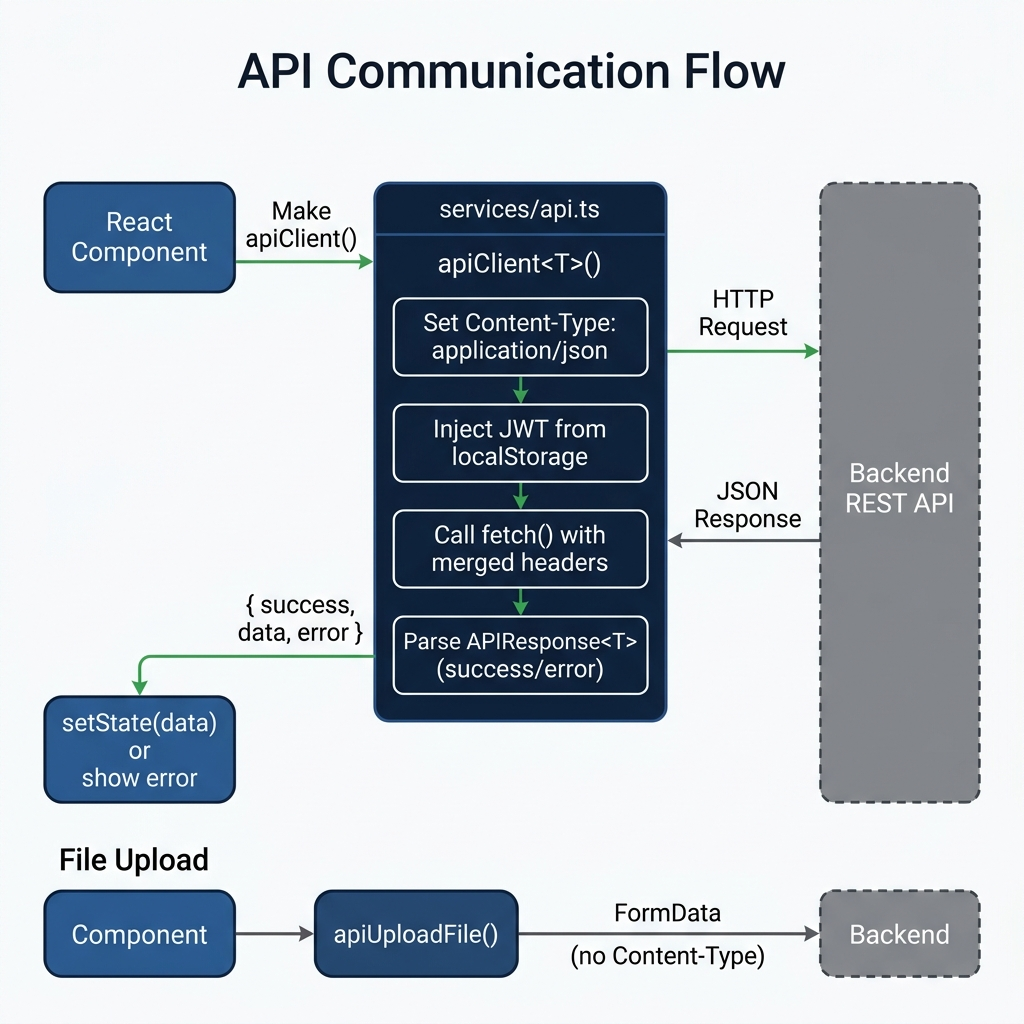
\includegraphics[width=\textwidth]{images/api_flow_diagram.png}
    \caption{API request flow — all requests go through the centralized apiClient.}
\end{figure}

\subsection{The Custom \texttt{apiClient<T>()} Request Wrapper}

\begin{lstlisting}[language=TypeScript,title={api.ts — Comprehensive API Client}]
export interface APIResponse<T = any> {
  success: boolean;
  data: T | null;
  error: string | null;
}

export const API_BASE_URL = process.env.NEXT_PUBLIC_API_URL || "http://localhost:8000/api/v1";

export async function apiClient<T>(
  endpoint: string,
  options: RequestInit = {}
): Promise<APIResponse<T>> {
  try {
    const defaultHeaders: HeadersInit = {
      "Content-Type": "application/json",
    };

    if (typeof window !== "undefined") {
      const token = localStorage.getItem("access_token");
      if (token) {
        defaultHeaders.Authorization = `Bearer ${token}`;
      }
    }

    const response = await fetch(`${API_BASE_URL}${endpoint}`, {
      ...options,
      headers: {
        ...defaultHeaders,
        ...options.headers,
      },
    });

    const data = await response.json();
    
    if (data && typeof data.success !== 'undefined') {
        return data as APIResponse<T>;
    }

    if (!response.ok) {
      return { success: false, data: null, error: data.error || "Request failed" };
    }

    return { success: true, data: data.data, error: null };
  } catch (error: any) {
    return { success: false, data: null, error: error.message || "Network error" };
  }
}
\end{lstlisting}

\subsection{Architectural Decisions and Advantages}

Decoupling API structures into a customized wrapper client yields three primary technical benefits:
\begin{enumerate}[leftmargin=2em]
    \item \textbf{Centralized Boundary Gateway for REST Operations:} The role of `apiClient` is to act as a secure gatekeeper and proxy for all backend REST communications across both student and admin layouts.
    \item \textbf{Compile-Time Generic Type Safety and Bundle Optimization:} Traditional SPAs often load heavy network clients (such as Axios), increasing the JS bundle footprint. Native `fetch` is performant and integrates with the Next.js cache. Enforcing a generic boundary (\texttt{<T>}) propagates strict compile-time types directly from the network layer to React state hooks.
    \item \textbf{Stateless Authorization Injection and Server-Side Safety:} Next.js server components render page structures on the backend, where client browser objects (like \texttt{localStorage} and the global \texttt{window} context) are unavailable. Calling \texttt{typeof window !== "undefined"} ensures safety during compilation. If the script executes in a browser environment, it retrieves the client's JWT token, injects the Bearer authorization header dynamically, and parses JSON payloads uniformly.
\end{enumerate}

\subsection{Handling Multipart Binary File Uploads}

Uploading housing application documents (PDFs or images) requires a separate multipart uploader:

\begin{lstlisting}[language=TypeScript,title={api.ts — Multipart uploader}]
export async function apiUploadFile<T>(
  endpoint: string,
  formData: FormData
): Promise<APIResponse<T>> {
  try {
    const headers: HeadersInit = {};
    
    if (typeof window !== "undefined") {
      const token = localStorage.getItem("access_token");
      if (token) {
        headers.Authorization = `Bearer ${token}`;
      }
    }

    const response = await fetch(`${API_BASE_URL}${endpoint}`, {
      method: "POST",
      headers,
      body: formData,
    });

    const data = await response.json();
    return { success: true, data, error: null };
  } catch (error: any) {
    return { success: false, data: null, error: error.message || "Upload failed" };
  }
}
\end{lstlisting}

\subsubsection{Technical Mechanics of FormData Uploads}

\begin{itemize}[leftmargin=2em]
    \item \textbf{Stateless Binary Data Upload Interface:} The role of this helper is to send binary document payloads (such as identity papers and student enrollment proofs) securely to the backend.
    \item \textbf{Content-Type Resolution and Header Omission Rules:} A common mistake in file upload services is setting the HTTP \texttt{"Content-Type"} header to \texttt{"multipart/form-data"} manually. When sending dynamic files, the browser must append a unique, randomized boundary string to delineate each file chunk in the request body (e.g., \texttt{Content-Type: multipart/form-data; boundary=----WebKitFormBoundaryX...}). 
    \item \textbf{Browser-Managed Boundary Construction and Execution Flow:} Manually setting this header overrides the browser's ability to append this boundary string, causing the backend to reject the request payload. Leaving the \texttt{Content-Type} empty instructs the browser to automatically set the correct header with its generated boundary, ensuring successful file transfers.
\end{itemize}

% ══════════════════════════════════════════════════════════
% SECTION 7: AUTHENTICATION & AUTHORIZATION
% ══════════════════════════════════════════════════════════
\section{Authentication \& Authorization Flow}

Protecting student applications and administrative housing actions is managed by an integrated authentication and role-based routing flow.

\begin{figure}[H]
    \centering
    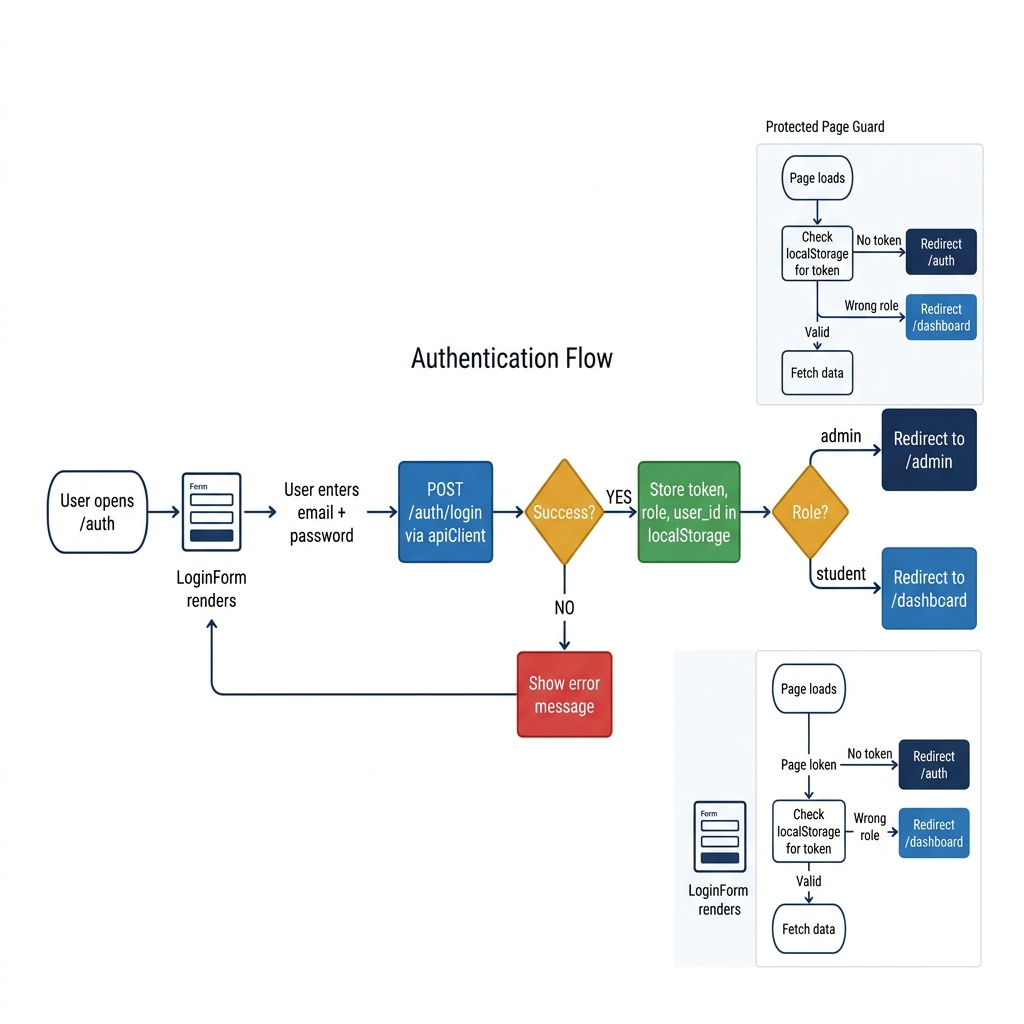
\includegraphics[width=\textwidth]{images/auth_flow_diagram.png}
    \caption{Authentication flow — from login to role-based routing to protected page guards.}
\end{figure}

\subsection{The Session Security Lifecycle}

\begin{enumerate}
    \item \textbf{Credential Verification:} The client enters credentials into the \texttt{LoginForm}. The component submits a `POST /auth/login` payload via the centralized `apiClient`.
    \item \textbf{Token Dispatch:} Upon successful verification, the backend issues a stateless JWT (JSON Web Token), which contains a cryptographic signature verifying the user's ID and role.
    \item \textbf{Client Storage:} The client receives the token and stores it in \texttt{localStorage} alongside the user's role:
    \begin{itemize}
        \item \texttt{access\_token:} The JWT string included in subsequent HTTP requests.
        \item \texttt{user\_role:} The system access role used for rapid route checking.
    \end{itemize}
    \item \textbf{Redirection:} The login handler inspects the role and redirects the user: admins to \texttt{/admin}, and students to \texttt{/dashboard}.
\end{enumerate}

\subsection{Client-Side Protected Route Guards}

To prevent unauthenticated users from accessing protected views, pages load layout route guards on mount inside a lifecycle `useEffect` hook:

\begin{lstlisting}[language=TypeScript,title={Protected route guard pattern (from app/admin/page.tsx)}]
"use client";
import { useEffect, useState } from "react";
import { useRouter } from "next/navigation";
import { apiClient } from "@/services/api";

export default function AdminPage() {
  const router = useRouter();
  const [authorized, setAuthorized] = useState(false);

  useEffect(() => {
    const token = localStorage.getItem("access_token");
    const role = localStorage.getItem("user_role");

    if (!token) {
      router.push("/auth");
    } else if (role !== "admin") {
      router.push("/dashboard");
    } else {
      setAuthorized(true);
    }
  }, [router]);

  if (!authorized) {
    return (
      <div className="min-h-screen flex items-center justify-center bg-background">
        <span className="material-symbols-outlined animate-spin text-primary text-4xl">
          refresh
        </span>
      </div>
    );
  }

  return (
    <div>
      {/* Real admin view contents */}
    </div>
  );
}
\end{lstlisting}

\subsubsection{Technical Mechanics of Client-Side Route Guards}

\begin{itemize}[leftmargin=2em]
    \item \textbf{Layout Protection Gate for Administrative Spaces:} The role of the route guard is to act as a secure gateway for protected layouts, verifying user roles and credentials before loading page modules.
    \item \textbf{Visual Flashing Mitigation for Unauthenticated Requests:} If the guard checked auth status asynchronously while the browser rendered the page, unauthenticated users might briefly see sensitive administrative data (layout flashing) before the redirect completes.
    \item \textbf{Lifecycle Mount Interception and State Synchronization:} The component initializes the local state variable \texttt{authorized} to \texttt{false}. The \texttt{useEffect} hook acts as a lifecycle gate. On mount, it reads the local storage token and user role. If invalid, it immediately invokes \texttt{router.push()} to redirect the user to the access portal. If authorized, it updates the state to \texttt{true}, unlocking the main layout.
\end{itemize}

% ══════════════════════════════════════════════════════════
% SECTION 8: INTERNATIONALIZATION (i18n)
% ══════════════════════════════════════════════════════════
\section{Internationalization (i18n) — Arabic \& English}

Because university housing serves diverse student demographics, the Sakny platform provides comprehensive bilingual support (English and Arabic), incorporating dynamic right-to-left layout transitions.

\begin{figure}[H]
    \centering
    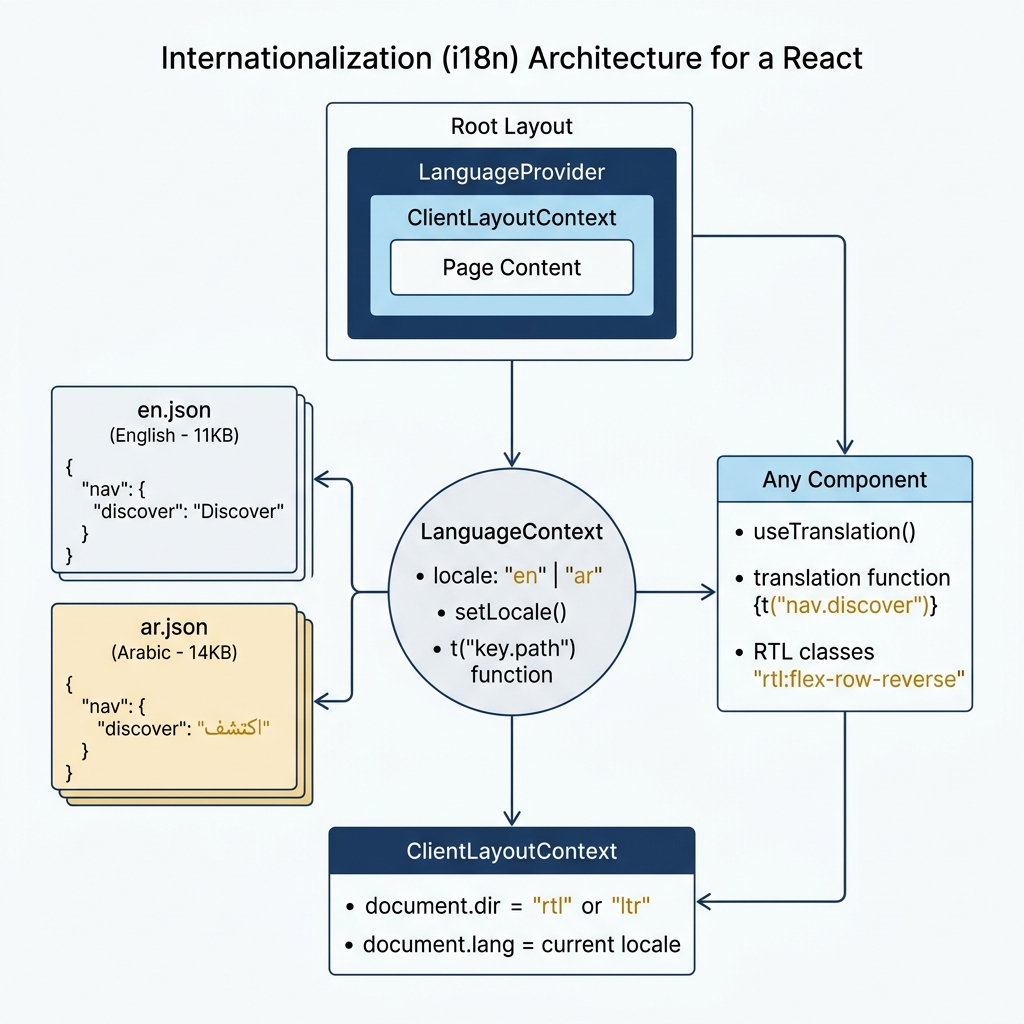
\includegraphics[width=0.9\textwidth]{images/i18n_architecture.png}
    \caption{i18n architecture — LanguageProvider supplies translations to all components via Context.}
\end{figure}

\subsection{Bilingual Context Architecture}

Rather than adding heavy third-party localization packages (like `react-i18next` or `next-intl`), the system uses a custom React Context provider. This lightweight solution minimizes bundle size and has zero runtime dependencies.

The localized strings are stored in structured JSON dictionary files inside `src/i18n/locales/`:

\begin{lstlisting}[language={},title={en.json (English translation dictionary snippet)}]
{
  "auth": {
    "loginButton": "Login",
    "fields": {
      "email": "Email Address",
      "password": "Password"
    }
  }
}
\end{lstlisting}

The context provider wraps the application DOM, providing translation lookups to child components:

\begin{lstlisting}[language=TypeScript,title={LanguageContext.tsx — Context provider and key resolver}]
"use client";
import React, { createContext, useState, useEffect } from "react";
import en from "./locales/en.json";
import ar from "./locales/ar.json";

type Locale = "en" | "ar";
const translations: Record<Locale, any> = { en, ar };

type LanguageContextProps = {
  locale: Locale;
  t: (key: string) => string;
  changeLanguage: (lang: Locale) => void;
};

export const LanguageContext = createContext<LanguageContextProps | undefined>(undefined);

export const LanguageProvider: React.FC<{ children: React.ReactNode }> = ({ children }) => {
  const [locale, setLocale] = useState<Locale>("en");

  useEffect(() => {
    const saved = localStorage.getItem("lang") as Locale;
    if (saved === "en" || saved === "ar") setLocale(saved);
  }, []);

  const changeLanguage = (lang: Locale) => {
    setLocale(lang);
    localStorage.setItem("lang", lang);
  };

  const t = (key: string): string => {
    const keys = key.split(".");
    let value: any = translations[locale];

    for (const k of keys) {
      if (value && typeof value === "object" && k in value) {
        value = value[k];
      } else {
        let fallbackValue: any = translations["en"];
        for (const fk of keys) {
          fallbackValue = fallbackValue?.[fk];
        }
        return fallbackValue ?? key;
      }
    }
    return value;
  };

  return (
    <LanguageContext.Provider value={{ locale, t, changeLanguage }}>
      {children}
    </LanguageContext.Provider>
  );
};
\end{lstlisting}

\subsection{Resolver Key Parsing Mechanics}

\begin{itemize}[leftmargin=2em]
    \item \textbf{Bilingual UI Context Resolution Engine:} The role of the custom provider is to supply a dynamic dictionary lookup function (\texttt{t()}) that intercepts visual text calls, returning translated strings based on the active locale.
    \item \textbf{Runtime Footprint Reduction and Dependency Optimization:} Heavy third-party internationalization packages add significant weight to client-side bundles. Developing a lightweight context provider keeps code simple and performant.
    \item \textbf{Dotted Path Extraction and Fallback Resolvers:} The translation resolver splits dot-notation lookups (e.g., \texttt{"auth.fields.email"}) into a string array: \texttt{["auth", "fields", "email"]}. It loops over the array, recursively traversing the active locale JSON object key by key. If the lookup fails (e.g., if a new Arabic translation is missing), the system catches the error and traverses the English fallback dictionary instead, avoiding layout crashes.
\end{itemize}

\subsection{RTL (Right-to-Left) DOM Layout Transitions}

Switching languages requires reflowing the visual DOM structures to align with the layout conventions of English (left-to-right) and Arabic (right-to-left). This transition is managed by the \texttt{ClientLayoutContext} component:

\begin{lstlisting}[language=TypeScript,title={ClientLayoutContext.tsx — Layout direction controller}]
"use client";
import React, { useEffect } from "react";
import { useTranslation } from "@/i18n/useTranslation";

export const ClientLayoutContext: React.FC<{ children: React.ReactNode }> = ({ children }) => {
  const { locale } = useTranslation();

  useEffect(() => {
    document.documentElement.dir = locale === "ar" ? "rtl" : "ltr";
    document.documentElement.lang = locale;
  }, [locale]);

  return <>{children}</>;
};
\end{lstlisting}

\subsubsection{Technical Alignment and Style Reflows}

\begin{itemize}[leftmargin=2em]
    \item \textbf{Dynamic Layout Direction Controller:} The role of this provider wrapper is to update the physical document layout direction parameters dynamically whenever the locale changes.
    \item \textbf{Native Browser Layout Reflow and Compilation:} Forcing directional changes via absolute JavaScript calculations causes browser jank and layout bugs. Leveraging the browser's native layout engine is faster and more reliable.
    \item \textbf{DOM Root Attribute Injection and Directional Style Mapping:} Updating the root \texttt{document.documentElement.dir} attribute triggers visual reflows in the browser's layout engine. Tailwind's compiler detects this change, dynamically applying classes prefixed with \texttt{rtl:} to mirror structural styles (e.g., padding alignments, floats, and flex directions) automatically.
\end{itemize}

% ══════════════════════════════════════════════════════════
% SECTION 9: CUSTOM HOOKS
% ══════════════════════════════════════════════════════════
\section{Custom Hooks}

Custom React hooks extract complex UI logic from page layouts into reusable functions, improving clean component design and maintainability.

\subsection{Intersection Observer Scroll Reveal Hook}

To build dynamic landing page experiences, the platform uses a custom \texttt{useScrollReveal} hook to trigger transition animations when elements scroll into view:

\begin{lstlisting}[language=TypeScript,title={useScrollReveal.ts — Performance-optimized animation hook}]
"use client";
import { useEffect, useRef, useState } from "react";

export function useScrollReveal(threshold = 0.1) {
  const ref = useRef<HTMLDivElement>(null);
  const [isVisible, setIsVisible] = useState(false);

  useEffect(() => {
    const observer = new IntersectionObserver(
      ([entry]) => {
        setIsVisible(entry.isIntersecting);
      },
      {
        threshold,
      }
    );

    const currentRef = ref.current;
    if (currentRef) {
      observer.observe(currentRef);
    }

    return () => {
      if (currentRef) {
        observer.unobserve(currentRef);
      }
    };
  }, [threshold]);

  return { ref, isVisible };
}
\end{lstlisting}

\subsubsection{Technical Rationale: Intersection Observer vs. Scroll Events}

\begin{itemize}[leftmargin=2em]
    \item \textbf{DOM Element Viewport Intersection Hook:} The role of the custom hook is to track element visibility within the viewport, toggling active animation states on the target layout elements.
    \item \textbf{Mitigation of CPU Execution and Scrolling Thread Blocking:} Legacy scroll animations listen to the window's scroll event, executing calculations on every single scroll tick. This blocks the main thread and causes UI jank. Using the browser-native \texttt{IntersectionObserver} offloads these visibility checks to the GPU thread, maintaining smooth 60fps animations.
    \item \textbf{Memory Allocation Management and Cleanup Lifecycle:} The hook binds a React \texttt{ref} to the target DOM node. When mounted, it initializes the native \texttt{IntersectionObserver} API. The browser monitors the element, executing the callback to update the local \texttt{isVisible} state when it crosses the viewport threshold. Returning a cleanup function that invokes \texttt{observer.unobserve()} ensures the observer is detached when the parent element unmounts, preventing memory leaks.
\end{itemize}

% ══════════════════════════════════════════════════════════
% SECTION 10: ERROR HANDLING & PERFORMANCE
% ══════════════════════════════════════════════════════════
\section{Error Handling \& Performance Optimization}

To maintain platform stability and high performance, Sakny implements standard error boundaries and performance optimizations at every layer of the frontend application.

\subsection{Resilient Error Handling Layer}

The frontend integrates structured error handling at the API, form, and page layers.

\subsubsection{API Response Resiliency}

The custom \texttt{apiClient} wrapper captures exceptions within standard \texttt{try/catch} blocks. If a server goes offline or a client suffers a connection timeout, the wrapper intercepts the exception and returns a formatted payload: \texttt{\{ success: false, data: null, error: "Network error" \}}. This prevents network errors from crashing React component execution.

\subsubsection{Client-Side Form Validation}

To reduce unnecessary server load, client-side input validations run on the client before firing requests over HTTP:

\begin{lstlisting}[language=TypeScript,title={LoginForm validation logic}]
const validate = () => {
  const newErrors: { email?: string; password?: string } = {};
  if (!formData.email) {
    newErrors.email = t("auth.errors.emailRequired");
  } else if (!/^\S+@\S+\.\S+$/.test(formData.email)) {
    newErrors.email = t("auth.errors.emailInvalid");
  }
  
  if (!formData.password) {
    newErrors.password = t("auth.errors.passwordRequired");
  }

  setErrors(newErrors);
  return Object.keys(newErrors).length === 0;
};
\end{lstlisting}

\paragraph{Form Validation Mechanics:}
\begin{itemize}[leftmargin=2em]
    \item \textbf{Client-Side Format Validation Controller:} The role of the validation function is to verify input formatting locally before initiating network connections.
    \item \textbf{Server Overhead Prevention and Latency Reduction:} Firing requests for malformed payloads increases backend database processing overhead. Catching errors locally saves server resources.
    \item \textbf{Regular Expression Verification and Interface Error Binding:} The helper uses regex patterns to validate fields. If a check fails, the function registers the issue inside the local \texttt{errors} state hook. This state maps directly to the input's \texttt{error} prop, instantly rendering visual warnings on the affected field.
\end{itemize}

\subsubsection{State-Driven Skeleton Loaders}

Data fetching layouts show animated loading states while waiting for API responses, avoiding jarring layout shifts:

\begin{lstlisting}[language=TypeScript,title={Loading state skeleton pattern}]
{loading ? (
  <div className="grid grid-cols-1 md:grid-cols-3 gap-6 animate-pulse">
    {[1, 2, 3].map((i) => (
      <div key={i} className="h-64 bg-slate-200 rounded-2xl" />
    ))}
  </div>
) : (
  <CatalogGrid data={housingData} />
)}
\end{lstlisting}

\paragraph{Skeleton Loading Mechanics:}
\begin{itemize}[leftmargin=2em]
    \item \textbf{Visual Representation of Anticipated Layouts:} The role of these components is to display temporary, animated shapes that mirror the expected page structure while content is loading.
    \item \textbf{Layout Shifts Prevention and Content Layout Smoothness:} Jarring layout shifts during data fetches can cause users to misclick elements, degrading the user experience. Skeletons reserve layout space ahead of time.
    \item \textbf{Conditional Render Toggles and Selective Hydration:} The view layer uses a conditional render block driven by a local \texttt{loading} boolean hook. While loading resolves to \texttt{true}, the compiler mounts the skeleton components with pulsing animations (\texttt{animate-pulse}). Once the API promise resolves, the state updates to \texttt{false}, smoothly replacing the skeletons with the loaded catalog grid.
\end{itemize}

\subsection{Core Performance Optimizations}

\subsubsection{Optimized Next.js Media Handling}

Rather than loading raw images using standard HTML \texttt{<img>} tags, the platform adopts the Next.js \texttt{next/image} utility:

\begin{lstlisting}[language=TypeScript,title={Optimized Image Loader Component}]
import Image from "next/image";

<Image
  src="/images/building-hero.jpg"
  alt="Sakny Housing"
  width={800}
  height={600}
  priority
  className="rounded-3xl object-cover"
/>
\end{lstlisting}

\paragraph{Automated Optimization Mechanics:}
\begin{itemize}[leftmargin=2em]
    \item \textbf{Media Delivery Optimization and Asset Scaler:} The role of this component is to serve optimized visual images while maintaining fast initial page loads.
    \item \textbf{Media Compression Optimization and Bandwidth Protection:} Large, uncompressed images slow down FCP scores. Next.js solves this by automating media compression.
    \item \textbf{Dynamic Transcoding and Breakpoint Scaling:} Next.js detects device layouts and transcodes raw assets into modern, compressed web formats (like WebP or AVIF) on the fly, reducing byte sizes. It scales image dimensions to match the client's screen size and lazy-loads off-screen images dynamically, saving network bandwidth.
\end{itemize}

\subsubsection{Polling Loop Optimizations \& Callback Memoization}

To display up-to-date alerts without overloading the server, components implement background polling using React's \texttt{useCallback} hook:

\begin{lstlisting}[language=TypeScript,title={useCallback Polling Optimization}]
const fetchNotificationCount = useCallback(() => {
  apiClient<NotificationCount>("/notifications/count")
    .then((res) => {
      if (res.success && res.data) {
        setNotifCount(res.data);
      }
    });
}, []);

useEffect(() => {
  fetchNotificationCount();
  const interval = setInterval(fetchNotificationCount, 30000);
  
  return () => clearInterval(interval);
}, [fetchNotificationCount]);
\end{lstlisting}

\paragraph{Dynamic Polling and Cleanup Mechanics:}
\begin{itemize}[leftmargin=2em]
    \item \textbf{Asynchronous Background Polling Loop:} The role of this module is to run background updates, ensuring real-time notification alerts are updated without requiring user interaction.
    \item \textbf{Garbage Collection and Memory Leak Mitigation:} Setting up background intervals without proper garbage collection can cause memory leaks. If the user navigates away, the interval loop continues executing in the background, consuming CPU cycles and slowing down the application.
    \item \textbf{Callback Memoization and Interval Lifecycle Management:} The component wraps the fetching function in React's \texttt{useCallback} hook, memoizing the function reference across renders. The \texttt{useEffect} hook initiates the interval. Importantly, the hook returns a cleanup function that invokes \texttt{clearInterval()} to clear the interval when the component unmounts, preventing memory leaks.
\end{itemize}

% ══════════════════════════════════════════════════════════
% SECTION 11: KEY FEATURE PAGES WALKTHROUGH
% ══════════════════════════════════════════════════════════
\section{Key Feature Pages Walkthrough}

This section details how styling, routing, components, and internationalization integrate on the three key pages of the application.

\subsection{Landing Page (\texttt{/})}

The public landing page acts as the entry point, introducing students to housing options and platform features.

\subsubsection{Architectural Composition}

The landing page file acts as a clean layout wrapper, loading structured feature components that build the marketing experience:

\begin{lstlisting}[language=TypeScript,title={page.tsx — Landing page composition}]
export default function Home() {
  return (
    <>
      <Navbar />
      <TrustBanner />
      <main className="flex-grow flex flex-col gap-32 pb-32">
        <Hero />
        <FeaturesGrid />
        <HowItWorks />
        <AIFeatures />
        <FinalCTA />
      </main>
      <Footer />
    </>
  );
}
\end{lstlisting}

\subsubsection{Key Execution Mechanics}
\begin{itemize}[leftmargin=2em]
    \item \textbf{GPU-Accelerated Visual Reveals:} Every sub-section of the landing page uses the \texttt{useScrollReveal} hook to apply clean entry transitions dynamically as the user scrolls.
    \item \textbf{Bilingual Rendering:} Localized values resolve dynamically using the context-driven translation function \texttt{t()}, ensuring that English and Arabic render correctly.
    \item \textbf{Optimized Hero Assets:} The \texttt{Hero} banner loads optimized, lazy-loaded background images that are styled using rich Tailwind v4 gradient overlays for a polished aesthetic.
\end{itemize}

\subsection{Student Dashboard (\texttt{/dashboard})}

The Student Dashboard is the central workspace where students track their housing applications, check document submission status, and see deadlines.

\subsubsection{12-Column Responsive Layout Structure}

The page uses a 12-column grid to organize workspace sections and sidebars:

\begin{lstlisting}[language=TypeScript,title={DashboardPage.tsx — Layout structure}]
<div className="max-w-7xl mx-auto grid grid-cols-12 gap-8 px-4">
  <div className="col-span-12 lg:col-span-8 space-y-12">
    <WelcomeBanner />
    <DocumentStatusStepper currentPhase={documentPhase} />
    <UploadDocumentCard onUploadSuccess={handleUploadSuccess} />
    
    <section className="grid grid-cols-1 md:grid-cols-2 gap-6">
      <ActionCard icon="assignment" title={t("dashboard.myApplication")} />
      <ActionCard icon="search" title={t("dashboard.findHousing")} />
      <ActionCard icon="group" title={t("dashboard.roommateMatching")} />
      <ActionCard icon="support_agent" title={t("dashboard.maintenance")} />
    </section>
  </div>
  
  <div className="col-span-12 lg:col-span-4">
    <DeadlinesSidepanel />
  </div>
</div>
\end{lstlisting}

\subsubsection{Dynamic Stepper Logic \& Phase Calculation}

The \texttt{DocumentStatusStepper} component guides students through the document upload process, dynamically updating its visual state based on backend application phases:

\begin{lstlisting}[language=TypeScript,title={Stepper stage evaluation}]
const docs = res.data.documents;
if (docs.length === 0) {
  setDocumentPhase("upload");
} else if (docs.some(d => d.status === "pending")) {
  setDocumentPhase("under_review");
} else if (docs.every(d => d.status === "approved")) {
  setDocumentPhase("approved");
} else if (docs.some(d => d.status === "rejected")) {
  setDocumentPhase("rejected");
}
\end{lstlisting}

\paragraph{Calculated Stepper Mechanics:}
\begin{itemize}[leftmargin=2em]
    \item \textbf{State Simplification and Document Process Stepper:} The role of this evaluation logic is to calculate a single visual phase from the dynamic array of document states returned by the API.
    \item \textbf{Student Workflow Navigation and Clarity Optimization:} Displaying raw status strings for each document can confuse students. Combining these states into a simplified progress stepper gives students a clear, unified view of their application progress.
    \item \textbf{Document Object Array Iteration and Status Reduction:} The page fetches document metrics, passing the response payload to the state resolver. The resolver parses the array: if empty, it triggers the upload phase; if any document is pending review, it activates the pending step; if all are approved, the stepper completes, rendering the appropriate UI state.
\end{itemize}

\subsection{Messages Page (\texttt{/dashboard/messages})}

The messages page provides a clean, two-panel chat interface where students can communicate directly with housing administrators.

\subsubsection{Split-Panel Grid Layout}

The page uses a split grid to separate active conversations from compose forms:

\begin{lstlisting}[language=TypeScript,title={Messages page — Split panel layout}]
<div className="grid grid-cols-1 lg:grid-cols-3 gap-6 max-h-[700px]">
  <div className="lg:col-span-2 bg-white border border-slate-200 shadow-soft rounded-2xl flex flex-col">
    <div className="flex-1 overflow-y-auto p-6 space-y-4 max-h-[500px]">
      {messages.map((msg) => {
        const isMine = msg.sender_role === myRole && msg.sender_id === myId;
        return (
          <div key={msg.id} className={`flex ${isMine ? "justify-end" : "justify-start"}`}>
            <div className={`max-w-[70%] p-4 rounded-2xl ${
              isMine 
                ? "bg-primary text-white rounded-br-sm rtl:rounded-br-2xl rtl:rounded-bl-sm" 
                : "bg-slate-100 text-slate-800 rounded-bl-sm rtl:rounded-bl-2xl rtl:rounded-br-sm"
            }`}>
              <div className="text-sm leading-relaxed">{msg.body}</div>
              <div className="text-[10px] opacity-60 mt-1.5 flex justify-end">
                {new Date(msg.created_at).toLocaleTimeString([], { hour: '2-digit', minute: '2-digit' })}
              </div>
            </div>
          </div>
        );
      })}
    </div>
  </div>
  
  <div className="bg-white border border-slate-200 shadow-soft rounded-2xl p-6">
    <form onSubmit={handleSend} className="space-y-4">
      {/* Recipient selectors and send inputs */}
    </form>
  </div>
</div>
\end{lstlisting}

\subsubsection{Key Execution Mechanics}
\begin{itemize}[leftmargin=2em]
    \item \textbf{Chat Bubble Alignment:} Messages are aligned dynamically based on the sender's identity. The system evaluates the \texttt{isMine} flag to determine layout classes (\texttt{justify-end} with deep primary colors for outgoing messages, vs \texttt{justify-start} with light backgrounds for incoming messages).
    \item \textbf{Direction-Aware Border Radius:} Border radius styles are direction-aware to match reading habits. For example, outgoing messages shave the bottom-right corner in English layouts (\texttt{rounded-br-sm}), but shave the bottom-left corner in Arabic layouts (\texttt{rtl:rounded-bl-sm}) to ensure clean chat bubbles.
    \item \textbf{Container Scroll Boundaries:} Setting \texttt{max-h-[500px] overflow-y-auto} creates a scrollable message box. This locks the chat window dimensions, keeping UI heights consistent when loading long conversation histories.
\end{itemize}

% ══════════════════════════════════════════════════════════
% SECTION 12: SUMMARY
% ══════════════════════════════════════════════════════════
\section{Summary}

The Sakny frontend is built on a modern React architecture designed to provide a secure, performant, and bilingual user experience. Table 4 summarizes the key architectural details.

\begin{table}[H]
\centering
\begin{tabular}{@{}lp{8.5cm}@{}}
\toprule
\textbf{Architectural Aspect} & \textbf{Technical Implementation Details} \\
\midrule
Base Engine Framework & Next.js 16.2.4 with App Router routing architecture. \\
Typing Specification & TypeScript 5.x, providing static compile-time type safety. \\
Style Architecture & Tailwind CSS 4.x using compile-time utility styles. \\
Visual Tokens system & Semantic CSS variables configured via the Tailwind `@theme` directive. \\
Page Routing Pattern & File-system routing with nested layouts to preserve client-side states. \\
State Architecture & React Context API for internationalization, and local component states. \\
API Gateway Client & Centralized \texttt{apiClient<T>} using browser-native fetch. \\
Security Layer & JWT stored in client \texttt{localStorage} with client-side \texttt{useEffect} page guards. \\
Bilingual Support (i18n) & Custom Context translations context with fallback dictionaries and automated RTL layouts switching. \\
Animation Hook Logic & Custom `useScrollReveal` hook utilizing browser-native `IntersectionObserver`. \\
Visual Media Loading & Automated optimization using Next.js \texttt{next/image} and \texttt{display: "swap"}. \\
Component Tree Hierarchy & Clean modular architecture: Tier 1 UI Primitives $\rightarrow$ Tier 2 Feature Components $\rightarrow$ Tier 3 Composition Pages. \\
\bottomrule
\end{tabular}
\caption{Frontend architecture summary.}
\end{table}

This modular, type-safe architecture supports 30+ dynamic routes and 25+ reusable components, providing university students and administrators with a fast, secure, and fully bilingual platform.

\end{document}
